\chapter{Pathfinding}
''Civil War Nation'' benutzt ein in Zellen aufgeteiltes Spielfeld. Um die Bewegung der Figuren auf diesem Spielfeld zu erm"oglichen, m"ussen die g"unstigsten Pfade gefunden werden. Hierbei wird der ''Dijkstra Algorithmus'' eingesetzt, der von der aktuell ausgew"ahlten Figur die Entfernung zu allen anderen Zellen auf dem Spielfeld zu berechnen. Diese Entfernung wird wiederum benutzt um Aktionen mit begrenzter Reichweite, wie schie"sen, Granaten werfen, oder Laufen, auf ihre Verf"ugbarkeit zu "uberpr"ufen.
Der Dijkstra Algorithmus wurde gegen"uber dessen Erweiterung, den A*-Algorithmus gew"ahlt, da wir ungerichtet "uber den Graphen laufen m"ochten, und somit die Kosten zu allen umliegenden Knoten erhalten m"ochten.

In dem Bild sind alle verschiedenen Zelleinf"arbungen auf einmal zu sehen.
\begin{description}[]
	\item \textbf{Gelb mit Rand:} Aktuell ausgew"ahlte Figur
	\item \textbf{Blau:} Terrain in Bewegungsreichweite
	\item \textbf{Rot:} Terrain in Angriffsreichweite
	\item \textbf{Gelb:} Geplanter Pfad
	\item \textbf{Gr"un:} Zelle, "uber die sich die Maus aktuell befindet
\end{description}

\begin{figure}
	\centering
	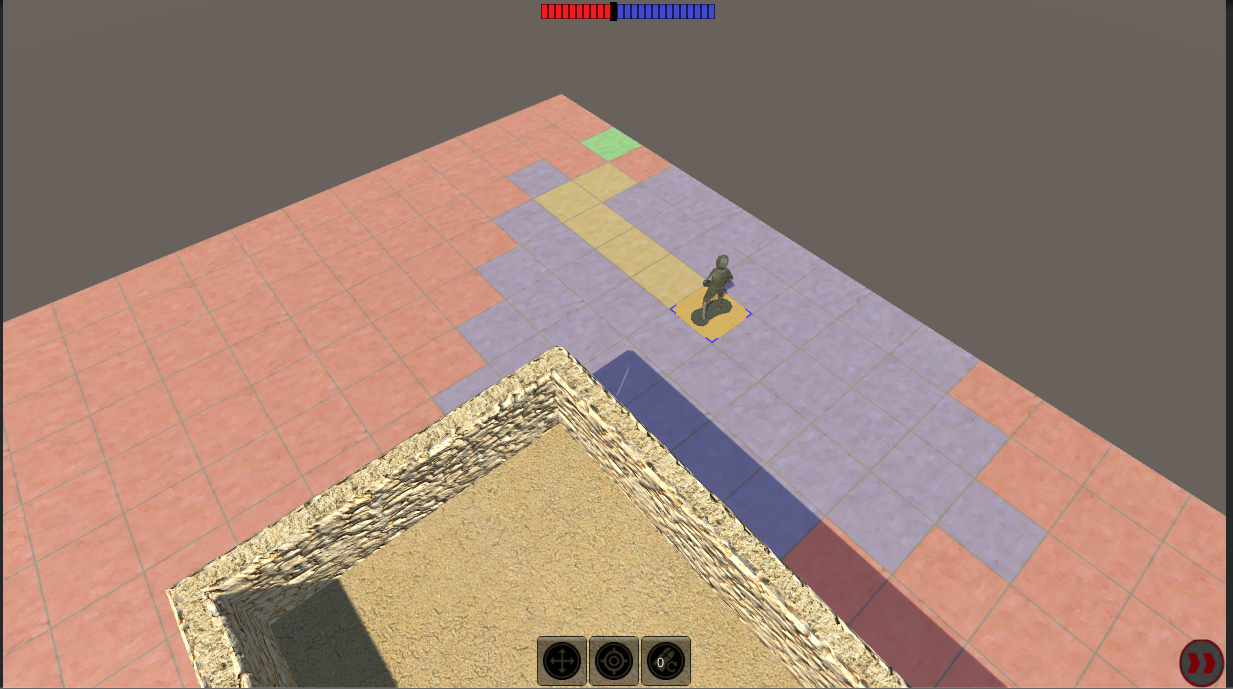
\includegraphics[height=6.5cm]{images/cell_info.png}
	\caption{Verschiedene Zelleinf"arbungen}
	\label{fig:cell_coloring}
\end{figure}